\newif\ifPhdDoc\PhdDoctrue
\newif\ifMonolithic\Monolithictrue
%\newif\ifTODO\TODOtrue                        % Use todo notes?

\newif\ifRootBuild\RootBuildfalse
\newif\ifOverLeaf\OverLeaffalse
\newif\ifIncludeWritingTips\IncludeWritingTipstrue
\ifMonolithic\else\newif\ifPhdDoc\PhdDoctrue
\newif\ifMonolithic\Monolithictrue
%\newif\ifTODO\TODOtrue                        % Use todo notes?

\newif\ifRootBuild\RootBuildfalse
\newif\ifOverLeaf\OverLeaffalse
\newif\ifIncludeWritingTips\IncludeWritingTipstrue


\documentclass[
uiophd
, 12pt
, english
, floatrow
%  , xelatex
, glossary                                     % Use a glossary
, biblatex                                 % Use a bibliography
%  , draft
%  , layout
, todos
]{common/mytemplate}
 

%\typeout{++++standalone++++}
%\usepackage[subpreambles=true]{standalone}

% \typeout{++++import++++}
% \usepackage{import}

% \typeout{--------------}
%\hypersetup{
%   bookmarksopen=true
% , bookmarksopenlevel=2
%}

\newcommand*\cleartoleftpage{%
	\clearpage
	\ifodd\value{page}\hbox{}\newpage\fi
}
% Fonts:
% https://tex.stackexchange.com/questions/19898/getting-urw-garamond-and-the-license

\providecommand*\paper[1]{}
\renewcommand*\paper[1]{{\bf{}Paper #1}}

\providecommand\1{}
\renewcommand*\1{\vec 1}
\providecommand\a{}
\renewcommand*\a{\vec a}
\providecommand\b{}
\renewcommand*\b{\vec b}
\providecommand\eR{}
\renewcommand*\eR{\mat{\hat R}}
\providecommand\eRi{}
\renewcommand*\eRi{\hat{\mat R}\;\!^{-1}}
\providecommand\k{}
\renewcommand*\k{\vec k}
\providecommand\n{}
\renewcommand*\n{\vec n}
\providecommand\p{}
\renewcommand*\p{\vec p}
\providecommand\R{}
\renewcommand*\R{\mat R}
\providecommand\Ri{}
\renewcommand*\Ri{\R^{-1}}
\providecommand\s{}
\renewcommand*\s{\vec s}

\providecommand\v{}
\renewcommand*\v{\vec v}
\providecommand\x{}
\renewcommand*\x{\vec x}
\providecommand\X{}
\renewcommand*\X{\mat X}
\providecommand\w{}
\renewcommand*\w{\vec w}

\providecommand\argmin{}
\renewcommand*\argmin[1]{\underset{#1}{\text{argmin}}\ }
\providecommand\norm{}
\renewcommand*\norm[1]{\left\lVert #1 \right\rVert}
\providecommand\min{}
\renewcommand*\min[1]{\underset{#1}{\text{min}}}
\providecommand\sinc{}
\renewcommand\sinc{\text{sinc}}

\providecommand*\nn{}
\renewcommand*\nn{\nonumber\\}

\providecommand\sumb{}
\renewcommand\sumb[2]{\sum\limits_{#1}^{#2}\;}

% \typeout{++++mylatexformat++++}
% \usepackage{mylatexformat}
\typeout{++++floatrow++++}
\usepackage{floatrow}
%\usepackage{bibtex}
%\usepackage{comment}
\typeout{++++environ++++}
\usepackage{environ}
%\usepackage[runin]{abstract}
\typeout{++++parskip++++}
\usepackage[parfill]{parskip}
\typeout{++++glossaries++++}
\usepackage[nonumberlist,nogroupskip]{glossaries}
\typeout{++++afterpage++++}
\usepackage{afterpage}
% \typeout{++++placeins++++}
% \usepackage{afterpage}
\typeout{++++subfiles++++}
\usepackage{subfiles}
%\typeout{++++standalone++++}
%\usepackage{standalone}
\typeout{++++subfig++++}
\usepackage[caption=false,font=footnotesize]{subfig}
\typeout{--------------}


% \newcommand\gls[1]{#1}

\renewcommand\figurename{Fig.}
\renewcommand\thefigure{\arabic{figure}}
\usepackage[margin=0pt,font={it,small},labelfont={bf,it},labelsep=colon]{caption}
% \addto\captionsenglish{\renewcommand{\figurename}{Fig.}}

\renewcommand\thetable{\arabic{table}} 
\renewcommand\theequation{\arabic{equation}} 

% Increase header a bit to allow two lines in it
\addtolength\headheight{\topmargin}
\setlength\topmargin{0pt}

\titleformat{\chapter}%command
[display]%shape
% {}%format
{\flushright}%format
{}%label
{0pt}%sep
{\color{Black}\bfseries\Huge}%before
[]%after
\titlespacing*{\chapter}{0pt}{*0}{*2}

\titleformat{\section}%command
[block]%shape
% {}%format
{\Large\bfseries}%format
{\thesection}%label
{10pt}%sep
{}%before
[]%after
\titlespacing*{\section}{0pt}{*0}{*0}

\titleformat{\subsection}%command
[block]%shape
% {}%format
{\large\bfseries}%format
{\thesubsection}%label
{10pt}%sep
{}%before
[]%after
\titlespacing*{\subsection}{0pt}{*0}{*0}

\addbibresource{../library.bib}
%\ifMonolithic
%\addbibresource{../HowtoHowtoCapon/library.bib}
%\fi

\renewcommand\include[1]{\subfile{#1}}

\vbadness=99999
\hbadness=99999

\endofdump
\begin{document}
	
\end{document}

\fi
%~~~~~~~~~~~~~~~~~~~~~~~~~~~~~~~~~~~~~~~~~~~~~~~~~~~~~~~~~~~~~~~~~~~~~~~~~~~~~~~~~~~~~~~~~~~~~~~~~~
\graphicspath{{../HowtoHowtoCapon/final/gfx/}}


\newcommand\IEEEmembership[1]{}

%\makeatletter
%\def\@maketitle{%
%%	\newpage
%%	\null
%%	\vskip 2em%
%%	\begin{center}%
%%		\let \footnote \thanks
%%		{\LARGE \@title \par}%
%%		\vskip 1.5em%
%%		{\large
%%			\lineskip .5em%
%%			\begin{tabular}[t]{c}%
%%				\@author
%%			\end{tabular}\par}%
%%		\vskip 1em%
%%		\abstracttext
%%		{\large \@date}%
%%	\end{center}%
%%	\par
%%	\vskip 1.5em
%}
%%\fi
%\makeatother


\titleformat{\chapter}%command
[display]%shape
% {}%format
{\flushright}%format
{}%label
{0pt}%sep
{\color{Black}\Huge\bfseries}%before
[]%after
\titlespacing*{\chapter}{0pt}{*0}{*2}

\providecommand\title[1]{} 
\renewcommand\title[1]{}

% \newcommand\title[1]{}
\providecommand\maketitle{}
\renewcommand\maketitle{}

% \titleformat{\chapter}[runin]{}
% {\put(-10,0){\color{SeaGreen}\Large\emph\thesection}}%  {\footnotesize \enspace \emph{Sec.}  }
%   {0pt}{\color{Black}\Large\bfseries\filright\textsl}[\vspace{15pt}\newline]
% \titlespacing*{\chapter}{0pt}{*4}{*0}


%\newcommand\title[1]{\makeatletter\def\mytitle{#1}\makeatother}
%\newcommand\maketitle{\makeatletter\meaning\@maketitle\makeatother}

\providecommand\author[1]{}
\renewcommand\author[1]{}

\providecommand\markboth[2]{}
\renewcommand\markboth[2]{}

% \newcommand\author[1]{}
%\newcommand\thanks[1]{}
% \renewcommand\markboth[2]{}

% \ifOPTbeamer
%\newenvironment{narrow}[2]{%
%	\begin{list}{}{%
%			\setlength{\topsep}{0pt}%
%			\setlength{\leftmargin}{#1}%
%			\setlength{\rightmargin}{#2}%
%			\setlength{\listparindent}{\parindent}%
%			\setlength{\itemindent}{\parindent}%
%			\setlength{\parsep}{\parskip}}%
%		\item[]}{\end{list}}

\renewenvironment{abstract}%
{\list{}{\footnotesize
\setlength{\topsep}{\parskip}%
\setlength{\leftmargin}{0pt}%
\setlength{\rightmargin}{0pt}%
\setlength{\listparindent}{\parindent}%
\setlength{\itemindent}{1cm}%\parindent
\setlength{\parsep}{\parskip}	
}%\rightmargin\leftmargin
\item[\textbf{Abstract ---}]\relax}
{\endlist}

% Options for the abstract package
%\setlength\absleftindent{0mm}
%\setlength\absrightindent{0mm}


%\newenvironment{IEEEkeywords}{}{}
%\excludecomment{IEEEkeywords}
\NewEnviron{IEEEkeywords}{
}

\newcommand\IEEEcompsoctitleabstractindextext[1]{#1}

\newcommand\IEEEdisplaynotcompsoctitleabstractindextext{}
\newcommand\IEEEpeerreviewmaketitle{}
%\renewcommand\maketitle{}

\renewcommand\AA{Å}

\newcommand\IEEEPARstart[2]{#1#2}

\newif\ifPeerReview\PeerReviewfalse              % Whether to create the PeerReview version or
% Journal version
\newif\ifOnlineColor\OnlineColortrue            % Compile online color version?
\ifOnlineColor
\newcommand\figPostfix{_online}              % Colored images online
\else
\newcommand\figPostfix{_bw}                  % Black and white in journal
\fi

\newif\ifCLASSOPTIONcompsoc\CLASSOPTIONcompsocfalse

\newif\ifCLASSOPTIONcaptionsoff\CLASSOPTIONcaptionsofffalse

\newcommand\appendices{\textsc{Appendix}}

\newenvironment{IEEEbiography}{}{}

%\let\Fig\undefined
\typeout{====Start of macro parse====}
\subimport{../HowtoHowtoCapon/}{macros}
\typeout{====done====}



%    \ifPhdDoc
%   \RequirePackage[
%      backend=biber
%    , style=ieee
%    , citestyle=ieee
% %   , defernums=true
% %   , doi=true
% %   , eprint=false
% %%    , sortlocale=
% %%   , style=authoryear-icomp
% %   , url=false
%    ]{biblatex}
%    \fi

\typeout{====ifMonolithic====}
\ifMonolithic\else
   \addbibresource{../HowtoHowtoCapon/library.bib}
\fi

\typeout{====Start document parse====}
\ifMonolithic\else\input{build/subheader.tex}\fi
%~~~~~~~~~~~~~~~~~~~~~~~~~~~~~~~~~~~~~~~~~~~~~~~~~~~~~~~~~~~~~~~~~~~~~~~~~~~~~~~~~~~~~~~~~~~~~~~~~~

\cleardoublepage
\chapter{Paper II}
\mbox{}\hfill\parbox{.9\linewidth}{\setlength\parskip{\baselineskip}

{\renewcommand\baselinestretch{1.1}
\Large\bf An Optimized GPU implementation of the MVDR Beamformer for Active Sonar Imaging}

J.I. Buskenes, J.P. Åsen, C.-I.C. Nilsen and A. Austeng

IEEE Journal of Oceanic Engineering\\
Volume 40, Issue 2, April 2015
}

\newpage
\pagestyle{empty}

\cleardoublepage
\pagestyle{fancy}
\thispagestyle{plain}
\fancyhead[LE]{\bf Paper II}
\fancyhead[RO]{\bf\flushright An Optimized GPU implementation of the\\ MVDR Beamformer for Active Sonar Imaging}

\begin{center}
{\Large\bf An Optimized GPU implementation of the MVDR Beamformer for Active Sonar Imaging}

J.I. Buskenes, J.P. Åsen, C.-I.C. Nilsen and A. Austeng
\end{center}

\newif\ifBS\BSfalse
\ifBS
% 
% \graphicspath{gfx/../}
%
\title{An Optimized GPU Implementation of the MVDR Beamformer for Active Sonar Imaging}%
%
\author{Jo~Inge~Buskenes,~\IEEEmembership{Student Member,~IEEE,} %
        Jon~Petter~\AA{}Åsen,~\IEEEmembership{Student Member,~IEEE,} %
        Carl-Inge~Colombo~Nilsen,~\IEEEmembership{Member,~IEEE,} %
        Andreas~Austeng,~\IEEEmembership{Member,~IEEE}%
\thanks{J. I. Buskenes, C.-I. C. Nilsen and A. Austeng are with the Department of Informatics, University of Oslo, 0316 Oslo, Norway.}%
\thanks{J. P. \AA{}sen is with MI-Lab, Norwegian University of Science and Technology, 7491 Trondheim, Norway.}% <-this % stops a space
% \thanks{Manuscript received April 19, 2005; revised January 11, 2007.}
}%
%
% The paper headers
\markboth{IEEE Journal of Oceanic Engineering}%
{A Robust and Optimized GPU Implementation of the MVDR beamformer}%
%
% Publishers ID mark:
%\IEEEpubid{0000--0000/00\$00.00~\copyright~2007 IEEE}
%
% use for special paper notices
%\IEEEspecialpapernotice{(Invited Paper)}
%
% for Computer Society papers, we must declare the abstract and index terms
% PRIOR to the title within the \IEEEcompsoctitleabstractindextext IEEEtran
% command as these need to go into the title area created by \maketitle.
\IEEEcompsoctitleabstractindextext{%


\begin{abstract}%
% Two limiting factors of modern phased array sonar imaging systems are the angular resolution and contrast. Adaptive beamformers target these limitatitons by weighting sensors dynamically to fit the impinging wavefield.
%
The minimum variance distortionless response (MVDR) beamformer has recently been proposed as an attractive alternative to conventional beamformers in active sonar imaging. Unfortunately, it is very computationally complex because a spatial covariance matrix must be estimated and inverted for each image pixel. This may discourage its use unnecessarily in sonar systems which are continuously being pushed to ever higher imaging ranges and resolutions.

In this study we show that for active sonar systems up to 32 channels, the computation time can be significantly reduced by performing arithmetic optimizations, and by implementing the MVDR beamformer on a graphics processing unit (GPU). We point out important hardware limitations for these devices, and assess the design in terms of how efficiently it is able to use the GPU's resources. On a quad-core Intel Xeon system with a high-end Nvidia GPU, our GPU implementation renders more than a million pixels per second (1\;MP/s). Compared to our initial central processing unit (CPU) implementation the optimizations described herein led to a speedup of more than two orders of magnitude, or an expected five to ten times improvement had the CPU received similar optimization effort. This throughput enables real-time processing of sonar data, and makes the MVDR a viable alternative to conventional methods in practical systems.
% If the HISAS1030 was attached to a platform traveling at 1.8m/s, creating full-coverage sectorscan images in real-time would be possible with this performance.

% We benchmarked optimized implementations of the MV beamformer in MATLAB and C, running on a quad-core Intel Xeon E5620, and in CUDA running on a high-end nVidia card. The beamformers operated on data from the 32x4 element Kongsberg Martime HISAS1030 sonar, using a conservative set of robustification parameters. 
%The CPU would then be free to take on the rest of the beamforming as well.
\end{abstract}%
%
% Keywords (normally not used for peer reviews)
\begin{IEEEkeywords}
Adaptive beamforming, MVDR, Capon, sonar, active sonar, GPU, graphics processing unit, complexity.
\end{IEEEkeywords}
}%

% make the title area
\maketitle

% This command fixes abstract positioning for compsoc articles:
\IEEEdisplaynotcompsoctitleabstractindextext

% (Optional) Add some extra info on cover page of peer review papers:
% \ifCLASSOPTIONpeerreview
% \begin{center} \bfseries EDICS Category: 3-BBND \end{center}
% \fi

% Insert page break and insert second title (peer review mode)
\IEEEpeerreviewmaketitle

\maketitle

\section{Introduction}

% Images from a phased array active sonar system are formed in the post-processing by focusing on one pixel at a time. This is achieved by delaying and weighting each of the array's channels, providing coarse and fine adjustments to the region of focus, respectively. This is commonly referred to as beamforming. Assuming far-field conditions, the delays are usually chosen to steer the pixel of interest to broadside, and the weights chosen to reject the noise impinging on the array from non-broadside directions.
% 
% The algorithm responsible for carrying out this task is referred to as a beamformer. Depending on whether data is evaluated when choosing a suitable set of delays and weights, beamformers can be branded either conventional or adaptive. A good example of the former is the The Delay-and-Sum (DAS) beamformer, which - as the name implies - simply delay the sensor channels appropriately prior to summing them up. Applying various weight sets, or windows, to the data prior to summation allows the lateral \gls{SNR} to be improved, but at the inevitable expense of a deteriorated lateral resolution. \todo{aka. the curse of physics.}
% 
% The Minimum Variance Distortionless Response (MVDR) (or \gls{MVDR}) beamformer, have the potential to overcome this limitation. While ensuring unit gain in the look direction, it computes the set of weights that minimizes the energy accumulated by the array from other directions. In other words, whenever the distribution of noise and interference is primarily focused around specific angles, an array response with a high degree of suppression at these angles are chosen, resulting in an image with a lateral \gls{SNR} and resolution superior to anything the \gls{DAS} can come up with.


% 
% In active sonar imaging the constrast and resolution can be improved by the use of adaptive beamforming. 
% 
% Adaptive beamforming 
% A critical part in the sonar image formation is the 
% The image quality is mainly limited by beam pattern of the imaging arrays.  resolution and noise suppression
% 
% The quality of sonar images 
% 
% An essential part of a sonar imaging system is the beamformer. 
% 
% 
% A sonar image is typically formed by using receive beamforming to focus on one pixel at a time. The beamformer's ability to suppress interference   to focus on one pixel at the time. How well a pixel value is estimated, and thus how 
% 
% A sonar image is built one pixel at the time the 
% 
% The image quality of a sonar system will depend on the imaging arrays ability to focus in 
% 
% 
% 
% Forming images done by combining data from multiple receivers in a way that to obtain focus on one pixel at the time, and assigning the output value to the intensity of that pixel. The 
% 
% Most modern active sonar systems employ phased arrays to 
% The basic way of a sonar image was formed 
% 
% A sonar system's ability to 
% 
% Adaptive beamforming has 
% 
% The image quality 
% 
% To improve the image quality of 
% 
% In high resolution sonar imaging the 
% 
% The image 
% 
% 
% In a typical sonar imaging scenario an encoded signal is transmitted to highlight a surface of interest, and the reflected wavefield sampled using a receiver array. A image is then formed in the post-processing by coherently combining the receiver outputs to focus at one pixel at the time. The principle of adjusting the arrays focus is commonly referred to as beamforming, and involves assigning suitable delays and weights to the array's channels.
% 

% A sonar image is typically formed by using receive beamforming to focus on one pixel at a time.   The image resolution and contrast The image quality The quality of active sonar images depend - amoung other things - on the beamformer's ability to suppress interference  resolution and constrast
% 
% A sonar image is typically formed by using receive beamforming to focus on one pixel at a time. The quality of the final image will depend on the beamformer's ability to suppress interference and noise from off-pixel.    to focus on one pixel at the time. How well a pixel value is estimated, and thus how
% 
% 
% In conventional active sonar imaging systems 
% 
% Various methods have been applied to active sonar imaging. One of these methods, 
% 
%  eamforming techniques have been applied in several fields to improve image. methods can be applied to 
% 
% Most active sonar imaging systems are based on conventional beamforming methods. These are robust and simple, but does not take the incoming wavefield into account. offer  in the image formation process. While being inherently robust, these methods 
% 
% 
% With the ever increasing processing power found in modern computers 
% 
% As the processing power of todays modern computer systems keeps improving the feasibility of 
% 
% As the processing power of modern computer systems keep improving, the use of data adaptive methods in various imaging fields. 

\IEEEPARstart{D}{ata-driven} methods have been introduced in various imaging fields over the years in attempts to improve image quality. One such method is the minimum variance distortionless response (MVDR) beamformer. When compared to conventional methods, MVDR is often able to improve image contrast and resolution, as shown in, for example, radar~\cite{Benitz1997}, ultrasound~\cite{Synnevag2007}, and active sonar~\cite{Blomberg2013,Blomberg2012a,Dursun2009,Lo2004}.

Despite its inherent potential, the MVDR beamformer has yet to see widespread adoption in the active sonar field. There may be several reasons for this. For one, the method is not inherently robust, and may suffer from a phenomenon called signal cancellation in active systems~\cite{Widrow1982}. Another reason is that in its original form, the computational complexity is cubic with the number of channels, O($M^3$), while conventional beamformers are at O($M$). This is because a spatial covariance matrix is estimated and inverted for each image pixel.

% Robustification:
% R estimate accuracy vs. dynamic trackability: (1) Trade observation time for bandwidth (2) Partial adaptiveness (less degrees of freedom than channels) (3) Quadratic constraint on sensor weights to limit the norm to some preset value.
% -  
To ensure MVDR robustness, the literature suggests combining means such as temporal and spatial averaging, and regularization~\cite{VanTrees2002,Kailath1985}. On the other hand, the complexity issue can be handled by introducing well-founded approximations. For instance, some studies assume data stationarity which allows the formation of a Toeplitz-structured covariance matrix that is simpler to invert~\cite{Asl2012a,Jakobsson2000}. Other studies perform MVDR beamforming in beamspace (the spatial frequency domain), which can be considered sparse due to the limited angular extent of the received beam~\cite{VanTrees2002,Nilsen2009}. Exploiting this can lead to considerable performance improvements, especially in high channel count systems.

% Some low complexity approximations to the MVDR beamformer is also available, such as the Low Complexity Adaptive (LCA) beamformer, 

% Such devices can often this by combining up to thousands of computing cores that each performs modestly, but combined performs impressively. 

% We will show that by exploiting symmetry and avoiding unnecessary computations, the spatial averaging will also aid in reducing the overall arithmetic complexity\todo{make sure this is shown clearly somewhere}. for Unlike other work, which focus modifying or transforming\todo{get low channel count in, as it makes a case against the other solutions.} We make no approximations, but rather stay with a textbook example of the method that handle complex basebanded data\todo{misplaced?}.

% Other work (keywords: mvdr, capon, computation, efficient, complexity):
% - Partially adaptive beamforming. DAS on non-overlapping subarrays, then MVDR \cite{Swingler1999a}.
% - Beamspace / frequency based methods.
% - Low complexity. PCA + LC. 
% - Systolic arrays. Radar \cite{Ward1984} 
% - Toeplitz. \cite{Yapanel} Spectrum estimation - speech recognition. 
% 
% Us:
% - Aim for the GPU. Simple is often better.
% - Therefore: Optimize the standard MVDR chain.
% 1. Reduce arithmetic instructions
% 2. Implement for full utilisation of the arithmetic throughput on the GPU.
% 
% (Made partially adaptive by employing subarray averaging to reduce degrees of freedom to L.)


In this work, we show that such approximations may not be necessary for sonar systems up to 32 channels, since here the computation time can be reduced by one to two orders of magnitude by implementing MVDR on a graphics processing unit (GPU). Similar work may be found in, for example, medical ultrasound imaging, where Chen \emph{et al.} have demonstrated a GPU implementation of the MVDR that operates on real valued data~\cite{Chen2011,Chen2011a}. While this implementation is fast, the real valued data constraint does not allow the creation of asymmetric and shifted responses, and hence prevents the MVDR's potential to be fully reached. Our implementation is not restricted in this manner.

Our implementation is adapted to a well sampled 100\;kHz wideband active sonar system operating in the near field. The system has a range resolution comparable to the sampling period so our MVDR implementation runs in near single snapshot mode. To deal with this and to avoid signal cancellation we compute and average the covariance estimates from overlapping subarrays~\cite{Kailath1985}. This may resemble techniques such as "subarray MVDR"~\cite{Chapman1976}, but unlike that technique we are not using subarrays to reduce complexity but to make it feasible to use MVDR in an active system. In related work, we investigated using the same MVDR GPU implementation in cardiac ultrasound imaging~\cite{Asen2012,Asen2013}, and in active sonar imaging we have compared the performance of this implementation to comparable adaptive beamformers~\cite{Buskenes2013}.

This article is outlined as follows: In Section \ref{I_methods}, we introduce the concept of adaptive beamforming and provide details on the MVDR method. Then, in \ref{I_maptogpu}, we investigate the complexity issue, discuss means for reducing arithmetic complexity, and detail an implementation that makes efficient use of the GPU's parallel resources. The final design is assessed in Sections \ref{I_images_and_benchmarks} and \ref{I_discussion}, where we provide benchmarks, comparisons with similar CPU implementations, and measures of how efficiently our implementation makes use of the GPU's resources.

% Yay or nay? $\Rightarrow$ GPU ultrasound (\cite{So2011,Chen2011}). Complex data, all robustification techniques.



\section{Methods}\label{I_methods}

Consider a sonar imaging scenario where an encoded signal is transmitted to highlight a surface of interest, and assume that the backscattered wavefield is properly sampled using a uniform linear array of receivers. An image can then be formed by coherently combining the receiver outputs to focus at one angle at the time. The principle of adjusting the array's focus in range and direction is commonly referred to as beamforming, and involves assigning suitable delays and weights to the array's channels.


\subsection{Beamforming}
\ifPhdDoc
\begin{figure}[htbp]\centering
\includegraphics[width=\linewidth]{gfx/buske1\figPostfix.eps}
\else
\ifPeerReview
\begin{figure}[htbp]\centering
\includegraphics[width=0.8\linewidth]{gfx/buske1\figPostfix.eps}
\else
\begin{figure}[!t]\centering
\includegraphics[width=\linewidth]{gfx/beamforming.eps}
\fi\fi%
\caption{Beamforming principle. Signal signature is first removed by matched filtering. Then, before summation, a suitable set of delays $\Delta$ and weights $w$ are applied to focus on a pixel of interest at angle and range ($\theta,n$).}\label{I_beamforming}
\end{figure}
Let the receiver be an $M$ element uniform linear array, and assume that the signature of the transmitted signal has been removed by a matched filter (\Fig{I_beamforming}). Further assume that the array channels are digitally delayed to focus at a pixel with azimuth angle $\theta$ and range sample $n$, such that the delayed data from the $m$th channel can be expressed as $x_m[\theta,n]$. To simplify notation, we make the dependence on $\theta$ implicit from now on. 

By definition, the beamformer output $z[n]$ can now be expressed as the weighted sum of all the delayed data samples:
\begin{align}
z[n] = \w\H[n]\x[n] = \bmat{w_0[n]\\w_1[n]\\\vdots\\w_{M-1}[n]}^H \bmat{x_0[n]\\x_1[n]\\\vdots\\x_{M-1}[n]},\label{I_z}
\end{align}
where $w_m$ is the weight factor assigned to channel $m$. With static weights this would be referred to as the conventional delay-and-sum (DAS) beamformer. A large variety of weighting functions exists here for trading lateral resolution for improved noise suppression (contrast), but one always ends up with a compromise between the two~\cite{Harris1978}.

Various adaptive beamformers target this limitation by allowing the weights to change for each pixel to better fit the dynamic nature of the incoming wavefield. In other words, they attempt to use the \emph{a priori} information present in the data to improve image quality. The MVDR beamformer is one such method. It finds the set of complex weights that minimizes the beamformer's expected output power, while ensuring unity gain in the look direction~\cite{Capon1969}. This is a convex optimization problem that can be solved using Lagrange multipliers to yield the solution
\begin{gather}
\vec w[n] = \frac{\Ri[n]\a}{\a\T\Ri[n]\a},\label{I_weights}
\end{gather}
where $\a$ is a steering vector and $\R=E\{\x[n]\x\H[n]\}\in\mathbb{C}^{M,M}$ is the spatial covariance matrix for the full array. Since we pre-steer our data to every pixel in the image we simplify (\ref{I_weights}) by substituting $\a$ with a row vector $\1$ that represents broadside phase-steering. To estimate $\R$ we compute a sample covariance matrix $\eR$. In this computation we perform some degree of:
\begin{itemize}
\item \emph{spatial averaging} to avoid signal cancellation by decorrelating coherent echoes~\cite{Kailath1985};
\item \emph{temporal averaging} over an interval comparable to the pulse length (one to five samples) to maintain true speckle statistics~\cite{Synnevag2009};
\item \emph{diagonal loading} to improve robustness to parameter errors~\cite{Cox1987,Maksym1979}.
\end{itemize}%
%
% will perform some degree of \emph{spatial averaging} to avoid signal cancellation caused by coherent echoes~\cite{Kailath1985}, \emph{temporal averaging} to maintain true speckle statistics~\cite{Synnevag2009}, and \emph{diagonal loading} to improve robustness to parameter errors ~\cite{Cox1987,Maksym1979}. 
%
Combined, these steps will also ensure a numerically well conditioned $\eR$.

We perform \emph{temporal} and \emph{spatial averaging} first and put the result in an intermediate sample covariance matrix $\breve{\R}$. To do this we need to segment our array into subarrays. If we let $x_l[n]$ represent the data vector from subarray $l$ by
\begin{gather}
\x_l[n] = \bmat{x_l[n] & x_{l+1}[n] & \dots & x_{l+L-1}[n]}\T,
\end{gather}
then $\breve{\R}$ can be calculated as
\begin{gather}
\breve{\R}[n] =  \frac{1}{N_K N_L} \sumb{l=0}{M-L}\sumb{n'=n-K}{n+K} \x_l[n']\x_l\H[n'] \in\mathbb{C}^{L,L},\label{I_spatialR}
\end{gather}
where $N_K = 2K+1$ is the number of temporal samples to perform averaging over, and $N_L = M-L+1$ is the number of subarrays.

The final estimate $\eR$ is found by adding a fraction $d$ of the total power of $\breve{\R}[n]$ to its diagonal~\cite{Synnevag2007}:
\begin{align}
\eR[n] = \breve{\R}[n] + \I \frac{d}{L} \tr\{\breve{\R}[n]\},\label{I_finalR}
\end{align}
where $\I$ is an identity matrix, $\tr\{\cdot\}$ represents the matrix trace operation, and $\tr\{\breve{\R}[n]\}$ is an estimate of the energy received from this pixel.

Note how subarray averaging led to a size reduction of $\eR$ from $\mathbb{C}^{M,M}$ to $\mathbb{C}^{L,L}$, and hence will produce an $L$-element weight set when substituted into (\ref{I_z}). This weight set is applied to all the subarrays, before computing the beamformer output as in (\ref{I_z}). Or, equivalently, we may apply the weight set to the sum of all the subarrays by
%
\begin{align}
z[n] = \w\H[n] \sumb{l=0}{M-L} \x_l[n].\label{I_finalZ}
\end{align}
%
\ifPhdDoc
\begin{figure}[tbp]\centering
\includegraphics[width=\linewidth]{gfx/buske2\figPostfix.eps}
\else
\ifPeerReview
\begin{figure}[!t]\centering
\includegraphics[width=.8\linewidth]{gfx/buske2\figPostfix.eps}
\else
\begin{figure}[!t]\centering
\includegraphics[width=\linewidth]{gfx/implementation.eps}
\fi\fi%
\caption{MVDR beamforming. For each pixel in range and azimuth:\newline
1. an $L\times{}L$ sample covariance matrix $\eR$ is computed; \newline
2. the term $\eR^{-1}\1$ is found using a linear equation solver;\newline
3. and the beamformer output $z$ is computed from (\ref{I_finalZ}), where $\w$ is found by substituting $\eR^{-1}\1$ into (\ref{I_weights}). } \label{I_mvdr_beamforming}
\end{figure}
As summarized in \Fig{I_mvdr_beamforming}, the MVDR method is applied to each pixel independently, by:
\begin{enumerate}
\item computing the sample covariance matrix $\eR$ in (\ref{I_finalR});
\item computing $\eRi\1$ in (\ref{I_weights});
\item computing the beamformer output $z$ in (\ref{I_finalZ}).
\end{enumerate}
Next we will evaluate these steps in terms of arithmetic complexity, and then discuss their mappability to parallel hardware.

\subsection{Computational Complexity}

% \the\linewidth
 
% Computing and inverting $\eR$ is by far the most computationally intensive tasks in MVDR beamforming. This 

If we neglect spatial and temporal averaging, then the computation of $\eR$ is reduced to a single outer product with complexity of O($M^2$), and the inversion is then of O($M^3$). This might lead us to believe that the inversion step is by far the most complex. But if we implement spatial and temporal averaging as in (\ref{I_spatialR}), then computing $\eR$ is of O($N_K N_L L^2$) and the inversion of O($L^3$). Computing $\eR$ is now the most complex operation whenever $N_LN_K>L$.
%
\ifPhdDoc
\begin{figure}[tbp]\centering
\includegraphics[width=\linewidth]{gfx/buske3\figPostfix.eps}
\else
\ifPeerReview
\begin{figure}[!t]\centering
\includegraphics[width=.8\linewidth]{gfx/buske3\figPostfix.eps}
\else
\begin{figure}[!t]\centering
\includegraphics[width=\linewidth]{gfx/mvdr_complexity.eps}
\fi\fi%
\caption{Per-pixel computational complexity of the steps in MVDR beamforming (before any optimizations). To avoid signal cancellation in an active sonar system we usually set $L<\frac{M}{2}$, in which region the computation of $\eR$ dominates in terms of arithmetic complexity, especially when performing temporal averaging.}\label{I_mvdr_complexity}
\end{figure}
To visualize these relations, and include the effects of using complex numbers, we set up complexity formulas that account for the total number of arithmetic operations for each step in the MVDR process (see appendix \ref{I_mvdr_formulas}). The only excluded operation was partial pivoting used in the inversion step, but this should contribute marginally to the end result. The entire range of possible subarray sizes from $L\in[1,M]$ was finally evaluated, with temporal averaging set to $K\in\{0,1,2\}$, and the number of channels set to $M\in\{8,16,32\}$. The results are shown in \Fig{I_mvdr_complexity}.

Note how the computation of $\eR$ completely dominates at smaller subarray sizes, that solving $\eRi\1$ only plays a notable role for larger array and subarray sizes, and that the computation of $z$ has a negligible impact on computation time. Also notice how temporal averaging comes with a high computational penalty. This is because building $\eR$ is heavy on complex multiplications, which require three times as many arithmetic instructions as a complex addition, and a lot of these are repeated unnecessarily.


 

\section{Mapping the MVDR to a GPU}\label{I_maptogpu}


An important feature of MVDR beamforming, as with beamforming in general, is that each pixel can be computed independently and in an identical fashion. Furthermore, a typical sonar image may contain millions of pixels. This represents a level of data parallelism that appears very well suited for a massively parallel architecture such as the GPU.

We decided to investigate the feasibility of running MVDR on a GPU by mapping it to a Nvidia GeForce Quadro 6000, which performs similarly to the consumer grade Geforce GTX 480. This is a high-end Compute Unified Device Architecture (CUDA)-enabled GPU based on Nvidia's Fermi architecture, which as now been superseded by the Kepler architecture. The code was written in Nvidia's ``C for CUDA'' framework, which adds a few extra features to the C language to specify how to distribute work across a large number of threads. It would have been possible to use GPUs from AMD and the cross-platform OpenCL framework from the Khronos group instead, but CUDA has a batch linear equation solver~\cite{Nvidia} that no OpenCL library provides. As will be discussed later, this is a key component in our design.

To use Nvidia's own terminology, the Quadro 6000 comprises 14 streaming multiprocessors (SMs), each having 32 CUDA cores that execute a common program called a kernel. Combined these cores deliver a peak performance of more than 1\;Tflop/s (appendix \ref{I_throughput}). In practice this performance is hard to obtain, but one can get fairly close by balancing the load evenly on all cores, and by trying to avoid that some cores are forced to idle due to a pending data transfer or thread synchronization. As the steps in the MVDR method require different strategies for achieving this, we have designed a different kernel and configuration for each of them. We will pay particular attention to building $\eR$, since the potential for gaining overall speedups are greatest here.

%  this assumes that the implementation is solely bound by arithmetic throughput.  r bound by memory bandwidth, arithmetic latency or arithmetic bandwidth.  or  is solely bound by processing power.   These cores need to be kept busy if we are to That make for a total of 448 CUDA cores which we need to keep busy if we want to tap the full potential. 

\ifPhdDoc
\begin{figure}[tbp]\centering
\includegraphics[width=\linewidth]{gfx/buske4\figPostfix.eps}
\else
\ifPeerReview
\begin{figure}[t]\centering
\includegraphics[width=.8\linewidth]{gfx/buske4\figPostfix.eps}
\else
\begin{figure}[t]\centering
\includegraphics[width=\linewidth]{gfx/mvdr_build_R.eps}
\fi\fi%
\caption{Step 1: Building $\eR$. This is a visualization of how $\eR$ could be built in a case with $M=5$ sensors, with subarray size $L=3$ and temporal averaging set to $K=1$. Here $\R'_{l}$ is the sample covariance matrix for the $l$th subarray, and $\breve{\R}$ is the average of $N_K$ of these. Note that instead of performing the temporal sum last as here, one could take more temporal samples into consideration in the computation of each $r_{ij}$.}\label{I_mvdr_build_R}
\end{figure}


% Memory latency can be hidden in two ways. One is to keep a lot of threads queued up on each SM at all times, such that when some threads perform memory operations other threads can be scheduled to run instead. This is referred to as data level parallelism (DLP). Alternatively, or preferrably in addition, the designer may promote instruction level parallelism (ILP) by letting subsequent instructions in a thread be independent. While ILP can be very effective when done correctly, DLP is generally simpler to design for.

% load balancing
% - distribute load - optimize symmetry
% - avoid branching
% 
% memory latency hiding
% - make threads use high bandwidth memory
% - hide latency with dlp, ilp, or both
% 
% thread sync hiding
% - queue blocks up on an sm

%This is referred to as a single-program, multiple-data (SPMD) architecture\todo{malplaced}.

 %An SM is a single-program multiple-data (SPMD) processor, meaning that all the CUDA cores on an instruction unit, L1 cache and registers is shared by all the CUDA cores on that SM.  %
% GPUs, on the other hand, does not attempt to do ILP, but use all available transistors to support massive DLP. This leads to designs such as the nNvidia GeForce GTX 580. 
% each with 48kB of L1 cache (shared memory) and 128kB of register memory.

% -bank conflicts when L > 32. not treated.


\subsection[Computing the Spatial Covariance Matrix]{Computing the Spatial Covariance Matrix, $\hat{\boldsymbol{R}}$}\label{I_computing_eR}

% As \Fig{I_mvdr_complexity} illustrates the computation of $\eR$ 

As observed in \Fig{I_mvdr_complexity}, a direct computation of $\eR$ by implementing (\ref{I_spatialR}) and (\ref{I_finalR}) is the greatest computational burden. We target this issue by first minimizing arithmetic operations, then aim to get as close to the peak arithmetic throughput on the GPU as possible.

\subsubsection{Minimizing Arithmetic Operations}

In \Fig{I_mvdr_build_R}, we illustrate how to reduce the arithmetic complexity of building $\eR$ in a system with $M=5$ sensors, a subarray size of $L=3$, and temporal averaging is set to $K=1$. Here the spatial sum is carried out before the temporal sum. To reduce arithmetic operations we may:
%
\begin{enumerate}
\item exploit the fact that $\eR$ is Hermitian positive semidefinite to compute only one half of it;
\item avoid redundant multiplications;
\item avoid redundant summations by first computing the upper row of $\eR$ and then adding/subtracting to these iteratively to find the diagonals of $\eR$.
\end{enumerate}

\ifPhdDoc
\begin{figure}[tp]\centering
\includegraphics[width=\linewidth]{gfx/buske5\figPostfix.eps}
\else
\ifPeerReview
\begin{figure}[!t]\centering
\includegraphics[width=.8\linewidth]{gfx/buske5\figPostfix.eps} 
\else
\begin{figure}[!t]\centering
\includegraphics[width=\linewidth]{gfx/buildR-breakdown.eps}
\fi\fi%
\caption{Arithmetic optimization of computing $\eR$: Relative reduction in arithmetic complexity compared to the initial implementation shown in \Fig{I_mvdr_complexity} (higher is better). Note how the arithmetic count is reduced by a factor 4-10 in the memory-optimized case, and by a factor 6-22 in the instruction-optimized case.}\label{I_mvdr_complexity_optimized}
\end{figure}

To study the effect of these optimizations we altered the complexity formulas to take them into account. Exploiting symmetry and performing iterative summing (step 1 and 3) is always desirable, but avoiding redundant multiplications (step 2) comes at the cost of increased memory consumption. When all optimizations are applied, we call it a "minimum instructions" solution, and when step 2 is left out, we call it a "minimum memory" solution. \Fig{I_mvdr_complexity_optimized} compares the two solutions, and formulas may be found in Appendix \ref{I_mvdr_formulas}. Here the complexity curves are relative to the reference implementation in \Fig{I_mvdr_complexity}. Both solutions reduce the complexity considerably, and recomputing the multiplications does not make that much of a difference. We selected the memory minimized version since our algorithm is severely memory bound, as we will see next.

\ifPhdDoc
\begin{figure}[p]\centering
\includegraphics[width=.997\linewidth]{gfx/buske6\figPostfix.eps}
% Caption is the same, but using newlines for the items in it (since it is now on a page)
\caption{MVDR implemented on a GPU. We do this in 3 steps, where each step process the full image before moving on to the next step. \\[.5\baselineskip]\textbf{Step~1}: The sample covariance matrix $\eR$ is formed by threads running along its diagonals. This allows spatial averaging to be implemented in a computationally efficient manner and minimizes interthread communication.
\\[.5\baselineskip]\textbf{Step~2}: $\eRi\1$ is computed using the heavily optimized batched linear equation solver from Nvidia~\cite{Nvidia}. 
\\[.5\baselineskip]\textbf{Step~3}: The beamformer output $z$ is computed in a straightforward fashion using $L$ threads that first sum the subarrays and then apply the MVDR weighting function. A single thread finally sums all the channels up.}\label{I_mvdr_implementation}
\else
\ifPeerReview
\begin{figure}[!t]\centering
\includegraphics[width=.8\linewidth]{gfx/buske6\figPostfix.eps}
\else
\begin{figure}[!t]\centering
\includegraphics[width=\linewidth]{gfx/mvdr_implementation.eps}
\fi
\caption{MVDR implemented on a GPU. We do this in 3 steps, where each step process the full image before moving on to the next step. \emph{Step~1}: The sample covariance matrix $\eR$ is formed by threads running along its diagonals. This allows spatial averaging to be implemented in a computationally efficient manner and minimizes interthread communication. \emph{Step~2}: $\eRi\1$ is computed using the heavily optimized batched linear equation solver from Nvidia~\cite{Nvidia}. \emph{Step~3}: The beamformer output $z$ is computed in a straightforward fashion using $L$ threads that first sum the subarrays and then apply the MVDR weighting function. A single thread finally sums all the channels up.}\label{I_mvdr_implementation}
\fi%
\end{figure}

\subsubsection{Arithmetic Throughput}

When we compute $\eR$, we very rarely perform more than 1-3 floating point operations for every float read or written to memory. Unfortunately, the GPU prefers kernels to be more arithmetically intensive than this. This can be inferred from Table \ref{I_throughputs}, %
%
\begin{table}[!b]\centering%\normalsize
\begin{tabular}[c]{l r r r@{}  l}\hline
\rowcolor{tabBlue} & \multicolumn{1}{>{\columncolor{tabBlue}}c}{\bf B$_\text{arith}$} & \multicolumn{1}{>{\columncolor{tabBlue}}c}{\bf B$_\text{mem}$} & \multicolumn{2}{>{\columncolor{tabBlue}}c}{\bf B$_\text{mem}$/B$_\text{arith}$} \\\hline
Arithmetic & 1.03 Tflop/s & & &\\
Global memory & & 36 Gfloats/s & \hspace{30pt} 1 &:30 \\
Shared memory & & 257 Gfloats/s & 1 &:4 \\
Registers & & $>$1.5 Tfloats/s & $>$3 &:2~\cite{Vasilyy}
\end{tabular}
\caption{Nvidia Quadro 6000: Memory throughput, $B_{\lowercase{\text{mem}}}$, compared to arithmetic throughput, $B_\text{arith}$.}\label{I_throughputs}
\end{table}%
%
where the peak bandwidth of the three types of GPU memory are compared to the peak arithmetic throughput (see appendix \ref{I_throughput} for derivations). Global memory (RAM), in which all data must reside at some point, is at best only able to move one float for every 30 floats processed by the CUDA cores, and potentially much worse if care is not taken to use "coalesced" memory access patterns (that avoid memory bank conflicts). This is why the usage of global memory should be minimized. Shared memory, on the other hand, is a very fast level 1 cache that is shared by all threads on an SM. At peak performance, it is almost able to keep up with the computing units, but to obtain this performance we must make sure that:
\begin{enumerate}
\item the data needed to compute a pixel can fit in shared memory, while
\item the access patterns we use promote maximum bandwidth.
\end{enumerate}
 %Further alleviation is also possible by exposing instruction level parallelism within a thread, as this promotes the use of registers with a bandwidth at least 6 times higher than that of shared memory~\cite{Vasilyy}\todo{so why don't we? rephrase}.


These challenges are very closely linked. Since the Quadro 6000 architecture is of compute capability 2.0, it has 48\;kB shared memory (L1 cache) and 128\;kB of register memory per streaming multiprocessor (SM)~\cite{Nvidia2012}. This memory is shared by all active threads on that SM, a number that should be no less than 768~\cite{Nvidia2012a}. This is to expose a sufficient level of data parallelism to ensure that memory latency is completely hidden (in accordance with Little's law). If we divide the shared memory evenly on all 768 threads we find that each thread should store no more than 8 single precision complex numbers in shared memory, and 24 stored in registers. This should make it apparent why computing a single pixel per thread is a bad idea, and why we need to keep each thread as light on memory consumption as possible.

In \Fig{I_mvdr_implementation}, we illustrate how we get around these challenges. First we make each SM compute entire range lines of pixels, then load the subset of $\x$ that all these pixels depend upon into shared memory. This lets us perform temporal averaging without having to read additional channel data.

Second, we assign $L$ threads per pixel to traverse the diagonals of $\eR$. On the top row, a full computation is carried out, then that row is saved back to global memory following a coalesced access pattern that maximizes global memory bandwidth. For subsequent rows, the threads move along the diagonals while performing iterative summations; the result from the previous element on the diagonal is updated by adding and subtracting the correlation coefficients that enter and exit the sum, respectively. To minimize memory consumption, we compute the coefficients again every time we need them. When a thread has finished up a diagonal, we have them wrap around to compute one of the diagonals in the lower triangular of $\eR$. Since $\eR$ is conjugate symmetric, the values in the leftmost column are obtained by a complex conjugate copy of the relevant value in the first row. This is slightly nonoptimal as it causes divergent branching, but it is needed because the solver is Gauss Jordan based and thus require a full $\eR$. Combined these steps balance the load evenly on all threads, is almost completely free of arithmetic redundancy, and cause minimal memory consumption.
 

% \cite{Owens2007}\todo{Find a good spot for these}

\subsection[Inverting R]{Solving $\hat{\boldsymbol{R}}$$\;\!^{-1}$$\mathbf{1}$}

As intuition might suggest the matrix product $\eRi\1$ can be carried out by first inverting the matrix $\eR$, then performing the inner product with $\1$. However, one can also solve the linear equation $\hat{\boldsymbol{R}}\boldsymbol{b} = \1$ for $\boldsymbol{b}$, where $\boldsymbol{b} = \eRi\1$. This is the preferred approach since the solution is obtained directly and without the added computational cost of the final inner product.

An important thing to note here is that unlike the problems most GPU libraries try to solve, we do not attempt so solve large linear equations or invert large matrices; our matrices are small, but we have a very large number of them. Fortunately, Nvidia recently released a highly optimized batched linear equation solver tailored for this particular task. It is Gauss Jordan based and supports partial pivoting and complex numbers. The only downside to using it in our application is that it does not exploit the Hermitian property of our sample covariance matrix. A better choice would be a solver based on Cholesky decomposition. These are designed for Hermitian positive-semidefinite matrices such as our covariance matrix, and require only half the arithmetic operations of a Gauss Jordan solver.



\subsection[Computing z]{Computing $z$}

The beamformer output $z$ is computed on a per-pixel basis by first computing the MVDR weights $\w$, which are merely scaled versions of $\eRi\1$ (\ref{I_weights}). Then the sum in (\ref{I_finalZ}) is found by assigning a group of $L$ threads to respective elements of $x_l$, which then proceed to accumulate these for all $N_L$ subarrays. The resulting data vector is finally multiplied with the weight vector using the same threads, and then a single thread is used to sum these products to obtain $z$.

\subsection{Implementation summary}

% The GPU implementation can be summarized as follows:
% \begin{itemize}
% \item Pixels are processed in batches.
% \item Multiple threads per pixel.
% \item $\eR$ is computed directly from raw data to minimize memory footprint.
% \item Inversion step is performed by Nvidias batch linear equation solver.
% \item Design makes efficient use of cache and data transfers are kept to a minimum.
% \end{itemize}
% 
% We compare this to our CPU implementations, where:
% \begin{itemize}
% \item Pixels are processed one by one.
% \item Single thread per pixel.
% \item Computation of $\eR$ is optimized for minumum number of instructions, as in \ref{I_mvdr_build_R}. Only upper half of $\eR$ is computed (see next point).
% \item Inversion step carried out by a custom inline Cholesky based solver that only requires the upper triangular of $\eR$.
% \item Design has generally not been optimized for efficient use of memory.
% \end{itemize}

The GPU design is summarized and compared to our CPU designs in Table \ref{I_implementation_summary}.
%
\begin{table}[!ht]\centering%\normalsize
% \begin{tabular}[c]{l r r r@{}  l}\hline
\begin{tabular}[l]{l >{\raggedright}p{.27\linewidth} p{.28\linewidth}}\hline
\rowcolor{tabBlue} & \bf GPU & \bf CPU \\\hline
Pixel processing & In batches & One by one \\
Threads per pixel & Multiple & One \\
1. Building $\eR$:  & & \\
\ \ \ Values computed & All & Only upper triangular \\
\ \ \ Optimization    & Minimized memory consumption & Minimized number of instructions \\
2. Computing $\eRi\1$: & & \\
\ \ \ Method & Nvidia's batch\newline Gauss Jordan solver & Custom inline\newline Cholesky solver \\
Cache utilization & Efficient & Not efficient \\
Data transfers & Minimum & Moderate
\end{tabular}
\caption{Implementation summary.}\label{I_implementation_summary}
\end{table}


% There are essentially two ways to accelerate an algorithm on parallel hardware. One is to identify independent instructions for each thread, and run these in in parallel, and the other is to support the parallel execution of as many threads as possible. This is referred to as instruction level parallelism (ILP) and data level parallelism (DLP), respectively. Most general purpose processors, such as a CPUs, support both DLP by featuring multiple cores with single-data multiple-data (SIMD) capabilities, and ILP by through means such as branch prediction and out-of-order execution.

% GPUs, on the other hand, does not attempt to do ILP, but use all available transistors to support massive DLP. This leads to designs such as the nNvidia GeForce GTX 580. Using their own terminology, it is comprised of 16 ``streaming'' multiprocessors (SMs), each having having 32 CUDA\todo{make sure CUDA is introduced} cores that execute a common program called a kernel. %An SM is a single-program multiple-data (SPMD) processor, meaning that all the CUDA cores on an instruction unit, L1 cache and registers is shared by all the CUDA cores on that SM.  %
% each with 48kB of L1 cache (shared memory) and 128kB of register memory.




\section{Images and Benchmarks}\label{I_images_and_benchmarks}

To demonstrate the imaging capability of the MVDR beamformer, we have processed experimental datasets from the $M=32$ element Kongsberg Maritime HISAS1030 sonar mounted on a HUGIN autonomous underwater vehicle (AUV)~\cite{Hansen2009}. HISAS1030 is a high resolution synthetic aperture sonar (SAS) with an array length of 1.2\;m, operating frequency of 100\;kHz, and bandwidth of 30\;kHz. The element size and spacing is 2.5\;$\lambda$ and the opening angle is 25$^\circ$. To produce the image shown in \Fig{I_holmengraa}, the sonar was operated in sidescan mode. The studied object is the 1500-dwt oil tanker wreck Holmengraa. It is 68\;m long and 9\;m wide, and lies at a slanted seabed at 77\;m depth outside Horten, Norway. The 1 megapixel (MP) MVDR image was here processed with parameters $L=16$, $K=1$, and $d=1\%$.

\ifPhdDoc
\begin{figure}[tbp]\centering
\includegraphics[width=\linewidth]{gfx/buske7\figPostfix.eps}
\else
\ifPeerReview
\begin{figure}[!t]\centering
\includegraphics[width=.8\linewidth]{gfx/buske7\figPostfix.eps}
\else
\begin{figure}[!t]\centering
\includegraphics[width=\linewidth]{gfx/plot_holmengraa_L16_Navg1.eps}
\fi\fi%
\caption{HISAS sidescan sonar (SSS) image of the shipwreck Holmengraa that lies on a slanted seabed at 77\;m depth outside of Horten, Norway. The image was processed with $M=32$, $L=16$, $K=1$ and $d=1\%$. The image was linearly upinterpolated by a factor 2 in azimuth making its total size 1.46 megapixels (MP). Note how MVDR improves edge definition and reduces noise in shadow regions.}\label{I_holmengraa}
\end{figure}

The computational performance of our implementation was first assessed on a test system with a quad-core Intel Xeon E5620, 64\;GB of RAM and an Nvidia Quadro 6000 card. The results were obtained by processing a 1\;MP image from the data from a 32 channel array, for all subarray sizes $L$, and for $K\in\{0,1,2\}$. Runtime measurements are shown in \Fig{I_benchmarks}. The runtimes of memory-only and arithmetic-only GPU kernels are depicted in \Fig{I_code_assessment}. An estimate of computation efficiency is presented in \Fig{I_code_assess_flops}. We were also granted a test drive at the Boston HPC centre on a machine with an Intel Xeon E5-2670, 32\;GB RAM and an Nvidia K20. The results from this run are shown in \Fig{I_benchmarks_boston}.

\ifPhdDoc
\begin{figure}[p]\centering
\includegraphics[width=\linewidth]{gfx/buske8\figPostfix.eps}
% Same caption but slightly different formatting since it is now on its own page
\caption{\protect MVDR benchmarks. A 1\;MP image from a $M=32$ channel array was processed for all $L$, and for $K\in\{0,1,2\}$.
\\[.5\baselineskip]\textbf{Top:} The time the GPU spent on building $\eR$, solving $\eRi\1$, and computing $z$. Note the major speedup of building $\eR$ when compared to the complexity plot in \Fig{I_mvdr_complexity}.
\\[.5\baselineskip]\textbf{Bottom:} Compared to a reference MATLAB and single thread C implementation running on a CPU the GPU offered a speedup of 2-3 orders of magnitude, but these numbers are somewhat misleading. If the C implementation was properly optimized we expect the GPU to be no more than a factor 5-10 faster, even if its theoretical peak performance is ~20 times higher than that of the CPU.}\label{I_benchmarks}
\else
\ifPeerReview
\begin{figure}[!t]\centering
\includegraphics[width=.8\linewidth]{gfx/buske8\figPostfix.eps}
\else
\begin{figure}[!t]\centering
\includegraphics[width=\linewidth]{gfx/benchmark.eps}
\fi\caption{\protect MVDR benchmarks. A 1\;MP image from a $M=32$ channel array was processed for all $L$, and for $K\in\{0,1,2\}$.\newline \emph{Top:} The time the GPU spent on building $\eR$, solving $\eRi\1$, and computing $z$. Note the major speedup of building $\eR$ when compared to the complexity plot in \Fig{I_mvdr_complexity}.\newline
\emph{Bottom:} Compared to a reference MATLAB and single thread C implementation running on a CPU the GPU offered a speedup of 2-3 orders of magnitude, but these numbers are somewhat misleading. If the C implementation was properly optimized we expect the GPU to be no more than a factor 5-10 faster, even if its theoretical peak performance is ~20 times higher than that of the CPU.}\label{I_benchmarks}
\fi%
\end{figure}

\ifPhdDoc
\begin{figure}[p]\centering
\includegraphics[width=\linewidth]{gfx/buske9\figPostfix.eps}
\else
\ifPeerReview
\begin{figure}[!t]\centering
\includegraphics[width=.8\linewidth]{gfx/buske9\figPostfix.eps}
\else
\begin{figure}[!t]\centering
\includegraphics[width=\linewidth]{gfx/code_assessment.eps}
\fi\fi%
\caption{Execution time of an arithmetic-only and a memory-only version of the MVDR code. A dataset from an $M=32$ array was processed for all $L$ using $K=1$, and the mean execution time for a 1 megapixel (MP) image was used here. From this plot we can infer that the kernel building $\eR$ is memory bound, as the time the kernel spends performing memory transactions is higher than the corresponding time it spends carrying out arithmetical operations. Furthermore, when the total runtime is larger than the restricted kernels this can largely be attributed to latency, which we can see that building $\eR$ suffers from with the chosen parameters.}\label{I_code_assessment}
\end{figure}

\ifPhdDoc
\begin{figure}[p]\centering
\includegraphics[width=\linewidth]{gfx/buske10\figPostfix.eps}
\else
\ifPeerReview
\begin{figure}[!t]\centering
\includegraphics[width=.8\linewidth]{gfx/buske10\figPostfix.eps}
\else
\begin{figure}[!t]\centering
\includegraphics[width=\linewidth]{gfx/code_assess_flops.eps}
\fi\fi
\caption{\protect Code efficiency. An estimate of the number of floating point operations per second (Flop/s), found by dividing the theoretical complexity curves by actual run-times. This is a crude measure as it does not include any other instructions than the actual arithmetic operations in the MVDR computation.}\label{I_code_assess_flops}
\end{figure}

\ifPhdDoc
\begin{figure}[tbp]\centering
\includegraphics[width=\linewidth]{gfx/buske11\figPostfix.eps}
\else
\ifPeerReview
\begin{figure}[!t]\centering
\includegraphics[width=.8\linewidth]{gfx/buske11\figPostfix.eps}
\else
\begin{figure}[!t]\centering
\includegraphics[width=\linewidth]{gfx/benchmark_boston.eps}
\fi\fi
\caption{\protect MVDR benchmarks from Boston HPC centre with the new high-end Nvidia K20 Kepler GPU. The exact same scenario and code as in \Fig{I_benchmarks} was used here. With no code alterations the performance was only improved marginally compared to running on the Quadro 6000.}\label{I_benchmarks_boston}
\end{figure}

As seen in the runtime comparisons presented in \Fig{I_benchmarks}, the GPU method became two to three orders of magnitude faster than the C implementation we started out with. The remaining bottleneck in the final design is the inversion step, which is typically five times slower than the build step. In most cases the processing speed of the Quadro 6000 is above 1\;MP/s, and this was only improved by a factor 1.5-2 when run on the new K20 GPU. The benchmarks of our memory-only and arithmetic-only kernels show that the kernels spend roughly the same time on both these tasks, so optimising only one of these further will have marginal impact. All GPU kernels were compiled with \texttt{nvcc} at optimization level \texttt{O2}. Excluded from these benchmarks is the data transfer time from CPU to GPU, which account for 2-20\% of the total processing time. We believe it makes little sense to include them since it keeps getting easier to perform these data transfers in parallel by offloading the task to the direct memory access (DMA) controllers present on modern GPUs. Furthermore, the data rates in an active sonar are relatively low compared to the bandwidth available for these transfers.


\section{Discussion}\label{I_discussion}

In accordance with previous studies, \Fig{I_holmengraa} demonstrates the MVDR beamformer's ability to produce images with suppressed interference and improved detail resolution. Compared to the DAS beamformer, the ship's edges appear sharper and the shadows less noisy. In this scenario the MVDR's performance was not particularly sensitive to parameter adjustments. Similar performance was obtained with arbitrary combinations of $L\in\{12,16,24\}$, $K\in\{1,2,3\}$ and $d\in[0.01,0.05]$, and no adjustments had to be made when processing other parts of the scene.

As observed in \Fig{I_benchmarks}, the combination of minimizing arithmetic operations and implementing the MVDR on a GPU lead to a significant improvement in processing speed. Compared to a MATLAB and single thread C implementation, an order 2 and 3 speedup was achieved, respectively. Note that we do not consider this comparison fair. In fact, the theoretical peak throughput of this GPU is roughly 20 times higher than that the CPU in question, meaning the potential of the CPU was far from being reached in our initial implementations. The key reason for this is that the GPU design processes pixels in batches, which allows us to minimize data transfers and maximize the use of fast memory cache. In other aspects the designs are similar, both CPU implementations compute $\eR$ efficiently, and they make use of either an optimized custom Cholesky based solver or one from the Intel Math Kernel Library (MKL). Unfortunately we had little time to write a custom batch based solver and covariance builder for the CPU, but we expect the speed difference to be five to ten times, if we had compared two such designs.

Note from \Fig{I_benchmarks} how the building of $\eR$ now only takes up a fraction of the total processing time, and recall that it was the other way around when we presented the theoretical complexity curves in \Fig{I_mvdr_complexity}. Also, the benchmark curves for building $\eR$ now seem linear. The main reason for this is that the optimization step negated much of the extra complexity introduced by averaging, i.e., reduced the complexity from O($N_KN_LL^2$) to less than O($L^2$). Another reason for the runtime to appear more like O($L$) is likely that our design makes better use of the GPU's resources when there is more processing involved per pixel. The inversion step, on the other hand, gains less from being implemented on a GPU. This is because its nature is less data parallel. In particular, the back substitution step involved in its computation is mostly sequential. This difference can be observed in \Fig{I_mvdr_complexity}. Alternative solvers, such as one based on Cholesky decomposition that exploits the Hermitian property of $\eR$, can in theory reduce complexity by a factor two, but we question whether this result can be obtained in practice using a GPU. The CPU implementations perform Cholesky-based inversion, but this does not explain why the C and MATLAB implementation have a total runtime that is linearly dependent on $L$. We believe this happens because these implementations are dominated by the calculation of the covariance matrix and data movement, and not by the inversion step. 

When optimizing a GPU design it is important to know whether it is limited by memory bandwidth or arithmetical throughput. To measure this we made two versions of the MVDR kernel: One that only performs arithmetic operations, and one that only performs memory operations. Then, we benchmarked these kernels and compared their runtimes to the total runtime (\Fig{I_code_assessment}). A first thing to note is how these kernels seem equally occupied performing memory and arithmetic operations. This is a good sign, but since we consistently minimized memory consumption at the expense of some extra computations when building $\eR$ , we know it to be bound by memory bandwidth. It also has a problem with latency, which can be inferred from the total runtime being significantly higher than that of the two single-function kernels. Since the GPU hardware can carry out memory and arithmetic operations concurrently and independently, this gap indicates that the GPU sometimes does ``nothing''. In our case this is due to synchronization hold-ups when performing temporal averaging, which is carried out in a sequential manner.

Even with all our efforts we were unable to obtain processing rates higher than 40\;GFlop/s on average in the desirable range of subarray sizes (\Fig{I_mvdr_complexity}). This is mainly due to the inversion step, since for the most part we obtained more than 100\;GFlop/s when building $\eR$. While these numbers are slightly underestimated, they are regardless far away from the Quadro 6000's peak of 1\;TFlop/s. Again, we believe this is due to the design being bound by memory bandwidth. This belief is further supported by the test results from running the code on the new K20 Kepler card, where we saw a modest factor 1.5-2 speedup. Although the Kepler card peaks at 3.5-4\;Tflop/s, its shared memory bandwidth is only approximately twice that of the Quadro 6000, hence matches the observed speedup. However, it is likely that the Kepler card would perform better had we optimized our design for it. For scientific computing, the Kepler boards are considered more attractive, with the introduction of features such as kernels calling kernels, more registers, more shared memory, and better mechanisms for hiding or removing data transfers.


% If the HISAS1030 was attached to a platform moving at 1.8m/s, for which the maximum range is 250\;m~\cite{Hansen2010}, the pulse repetition frequency could be set to 3\;Hz. We could further assume a complex sampling frequency of 40\;kHz to accomodate the  HISAS1030's bandwidth of 30\;kHz, and beamform $M=32$ lateral beams. The throughput required for real-time processing of these images would then be 1\;MP/s. As we have seen, this is something our GPU implementation can handle if $L$ is not too large.\todo{droppe denne kanskje}%, leaving the \gls{CPU} free to take on other assignments.


% What may this performance be used for? Let us assume that the 32 element, 1.2\;m long HISAS1030 array is mounted on a platform moving at 1.8\;m/s. Then the pulse repetition frequency (PRF) could be set to 3\;Hz to ensure critical along-track sampling, 
% To illustrate what this performance might be used for, consider a moving platform travelling at 1.8\;m/s. 
% If the sonar system is Maximum range 
% There is a limit to the along-track sampli
% To avoid along track undersampling, the 

% HUGIN: 1.8m/s - range 250m \\
% fs = 100kHz*30\%*$\frac{4}{3}$ = 40kHz \\
% $N_{range px} = \frac{2\;250m}{1500m/s}40kHz = 13.3kpx$ \\
% $\times 32$ beams = 426kpx \\\\
% 
% PRF = $\frac{1500m/s}{2 250m} = 3Hz$ \\
% TP = 215px 3Hz = 1.28MP/s \\
% 4 arrays: 1.28MP/s * 4 = 5.12MP/s
% 
% 
% \begin{itemize}
% \item Need for speed: HUGIN 4 banks of 32 elements, can be processed faster than the ping repetition rate, with margins to spare.
% \end{itemize}


\section{Conclusion}\label{I_conclusion}

The MVDR beamformer is an algorithm capable of producing images with improved detail resolution and contrast compared to conventional DAS beamforming. The downside is its inherent need for robustification and the high computational complexity associated with estimating and inverting the spatial covariance matrix.

We have shown that for systems consisting of up to 32 channels the problem can be largely mitigated by building the covariance matrix in a clever way, and by making use of the massive computational power available in modern GPUs. We were able to improve upon the runtime of a single thread C-implementation by roughly two orders of magnitude. For most choices of parameters the GPU was able to create images at $\sim$1\;MP/s at an average data processing rate of $\sim$40\;GFlop/s. This is less than 5\% of the peak performance of the GPU, but we believe it to be near optimal given the constraints of memory bandwidth and the sequential nature of some parts of the MVDR implementation.

%  This performance is sufficient for computing properly sampled full-coverage sectorscan images from the HISAS1030 sonar in real-time.

All in all, the MVDR maps well to the GPU since the computations involved are independent on the pixel level, and partially also within each pixel. The GPU allows MVDR to be used in real-time processing of sonar data, and makes the MVDR a viable alternative to conventional methods in practical systems.


%%%%%%%%%%%%%%%%%%                              ~~~~~~~~~~~~~~~~~~~~~~~~~~~~~~~~~~~~~~~~~~~~~~~~~~
% DOCUMENT APPENDICES %
%%%%%%%%%%%%%%%%%%                              ~~~~~~~~~~~~~~~~~~~~~~~~~~~~~~~~~~~~~~~~~~~~~~~~~~


% \titleformat{<command>}[<shape>]{<format}{<label>}{<sep>}{<before>}[<after>]

% \titleformat{\section}[hang]{\bf}
% {\thesection.\enspace}%\thesubsubsection}%  {\footnotesize \enspace \emph{Sec.}  }
%    {0pt}{\MakeUppercase}[]
% \titlespacing*{\section}{0pt}{2\lineheight}{\lineheight}

% {-2ex plus -.5ex minus -.2ex}{1.0ex plus .2ex minus .2ex}

% \renewcommand\section[1]{{\Large\bf\MakeUppercase #1}}
% \renewcommand\section*[1]{{\Large\bf\MakeUppercase #1}}

% 
% 
% 
% 
% 
% 
% PRF = $\frac{1500m/s}{2 250m} = 3Hz$ \\
% TP = 215px 3Hz = 1.28MP/s \\
% 4 arrays: 1.28MP/s * 4 = 5.12MP/s
% 
% 
% 
% 1Tflops (ops/cycle?)
% 144GB/s global
% 1TB/s shared
% x6 regs
% 
% latency - arithmetic (20 cycles) and memory (400+ cycles)
% 
% Little's law - needed parallelism = latency * throughput
% arithmetic: 23 cycles * 32ops/SM/cycle = 576 ops/SM parallelism
% memory: <800 cycles * <144GB/s=125B/cycle = <100kB in the flight
% 
% On GF104: must have some ILP to get >0.66 of peak:
% - 48cores/SM, one instruction is broadcast across 16 cores
% - need 3 instructions per cycle
% - but only have 2 warp schedulers
% - instead, can issue 2 instructions per warp in the same cycle
% 

\ifPhdDoc
\clearpage
\renewcommand{\theHchapter}{A\arabic{chapter}}
\renewcommand{\theHsection}{A\arabic{section}}
\appendix
% \section*{Appendix}
\renewcommand\thesection{\Alph{section}}
\renewcommand\thesubsection{\Alph{section}.\arabic{subsection}}
\else
\appendices
\fi

\section{MVDR Complexity Formulas}\label{I_mvdr_formulas}

To estimate the number of floating point operations needed to MVDR beamform a single pixel, we formed expressions that accumulate the number of complex arithmetic operations found in the MVDR process. From observing the generated assembly code we inferred that each complex addition and multiplication would require $\Oa = 2$ and $\Om = 6$ floating point operations, respectively. The formulas are listed for each step below for reference.

\emph{Building $\eR$}. The initial complexity of this step can be inferred directly from (\ref{I_spatialR}) and (\ref{I_finalR}):
\begin{align}
O_{\underset{\text{initial}}{\text{Build $\eR$}}} &= \underbrace{\Om\Nk\Nl L^2}_\text{Multiplications} + \underbrace{\Oa(\Nk+\Nl-2)L^2}_\text{Additions} + O_\text{dload},
\end{align}
where $O_\text{dload} = (2L-1)\Oa + \Om$ is the minor cost of performing diagonal loading. If we apply the optimization strategies discussed in section \ref{I_computing_eR} we can arrive at the following instead:
\begin{align}
O_{\underset{\text{min arith}}{\text{Build $\eR$}}} &= \underbrace{\Om\frac{M+\Nl}{2}L}_\text{Multiplications} + \underbrace{\Oa(\Nk-1)(\Nl-1)L}_\text{First row additions} \nonumber\\
&+ \underbrace{\frac{(L-1)(L-2)}{2} \bigg[ 2\Oa + 2(\Nk-1)\Oa \Big]}_\text{Iteration additions} \nonumber\\
&+ O_\text{dload}
\end{align}
Of the solutions discussed, this is the least expensive in terms of arithmetic instructions. However, if memory bandwidth is a limiting factor a better solution is to recompute multiplications where they are needed:
\begin{align}
O_{\underset{\text{min mem}}{\text{Build $\eR$}}} &= \underbrace{\Om\Nk\Nl{}L}_\text{First row multiplications} + \underbrace{O_a(\Nk-1)(\Nl-1)L}_\text{First row additions} \nonumber\\
&+ \underbrace{\frac{(L-1)(L-2)}{2}\bigg[ 2\Oa + 2(\Nk-1)\Oa + 2\Nk\Om \bigg]}_\text{Iteration multiplications and additions} \nonumber\\
&+ O_\text{dload}.
\end{align}

\emph{Solving $\eRi\1$} is achieved by using a batched Gauss Jordan solver with support for complex numbers and partial pivoting. Its complexity, with partial pivoting excluded, can be expressed as: 
\begin{align}
O_{\text{Solve $\eRi\1$}} = \sumb{r=0}{L} \bigg[&\underbrace{\big(L-r\big)\big((L-r+2)\Oa + (L-r+3)\Om\big)}_\text{Reduction}\nonumber\\
+ &\underbrace{(r-1)\Oa + r\Om}_\text{Backsubstitution}\bigg],
\end{align}
where $r$ is a running variable $r$ that indexes rows in the augmented matrix $\bmat{\eR|\1}$.

\emph{Computing $z$} is very simple once the covariance matrix $\eR$ is built and inverted, and has an near negligible impact on performance: 
\begin{align}
O_\text{Compute $z$} = \Oa(2L-2)2 + \Om 3 L.
\end{align}



\section{GPU Throughput}\label{I_throughput}

In the context of determining whether an implementation is computationally bound or memory bound, one should first compare the target platform's sustained computational throughput to sustained memory throughput. Let us start with the former.

The Quadro 6000 has 32 CUDA cores per SM, each operating at a rate of 1148\;MHz and being able to perform 2 floating point operations (flop) per clock cycle when multiply-add instructions are used. The theoretical peak arithmetic throughput is then given as
\begin{align}
\text{B}_\text{arith} &= 2\cdot1148\;\text{Mflop/s/core}\cdot 32\;\text{cores/SM}\cdot 14\;\text{SMs}\nn
&= 1.03\;\text{Tflop/s}.\label{I_flops}
\end{align}
Now let us compare this to the memory throughput. The ``global'' GDDR5 memory bus is 384\;bit wide, and operates at 3\;Ghz where 2 bits are sent every cycle. Its peak bandwidth is then
\begin{align}
\text{B}_\text{gmem} &= \frac{2\cdot 3\;\text{Gbit/s}\cdot384\;\text{bit}}{8\;\text{bit/byte}}\nn
&= 144\;\text{GB/s}\ (36\;\text{Gfloats/s}).\label{I_bwglobal}
\end{align}
The shared memory, on the other hand, is organized into 32 banks per SM, each being 32\;bit wide and operating at 1148\;MHz where 1 bit is sent per cycle. Its peak aggregated bandwidth is then
\begin{align}
\text{B}_\text{smem} &= \frac{\frac{1148}{2}\;\text{Mbit/s}\cdot32\;\text{bit/bank}\cdot 32\;\text{banks/SM}\cdot 14\;\text{SMs}}{8\;\text{bit/byte}}\nn
&\approx 1.03\;\text{TB/s}\ (257\;\text{Gfloats/s}).\label{I_bwshared}
\end{align}
The bandwidths are compared in Tab. \ref{I_throughputs}. Note that even when using shared memory at least 4 floating point operations must be carried out per float transferred to the CUDA cores, otherwise the algorithm will be memory bound and the peak arithmetic throughput can not be reached.



%%%%%%%%%%%%%%%%%%                              ~~~~~~~~~~~~~~~~~~~~~~~~~~~~~~~~~~~~~~~~~~~~~~~~~~
% DOCUMENT APPENDICES %
%%%%%%%%%%%%%%%%%%                              ~~~~~~~~~~~~~~~~~~~~~~~~~~~~~~~~~~~~~~~~~~~~~~~~~~

\appendix

% use section* for acknowledgement
\ifCLASSOPTIONcompsoc% % This command fixes abstract positioning for compsoc articles:
% \IEEEdisplaynotcompsoctitleabstractindextext
% 
% % (Optional) Add some extra info on cover page of peer review papers:
% % \ifCLASSOPTIONpeerreview
% % \begin{center} \bfseries EDICS Category: 3-BBND \end{center}
% % \fi
% 
% % Insert page break and insert second title (peer review mode)
% \IEEEpeerreviewmaketitle
% 
% 
% 


  \section*{Acknowledgments}
\else
  \section*{Acknowledgment}
\fi


The authors would like to thank Kongsberg Maritime and the Norwegian Defence Research Establishment (FFI) for providing experimental data, and thank Nvidia for providing support on running the batched linear equation solver and for granting us a testdrive at the Boston HPC center.


% Can use something like this to put references on a page
% by themselves when using endfloat and the captionsoff option.
\ifCLASSOPTIONcaptionsoff
  \newpage
\fi



\ifPhdDoc
   \printbibliography[title=References,heading=subbibliography]
   \addcontentsline{toc}{section}{References}
%    \bibliographysty
%    \bibliography{library.bib}
%    \print
\else

% Originally build with bibtex:
% \bibliographystyle{IEEEtran}
% \bibliography{library.bib}

% Generated by IEEEtran.bst, version: 1.13 (2008/09/30)
\begin{thebibliography}{10}
\def\url#1{}
\csname url@samestyle\endcsname
\providecommand{\newblock}{\relax}
\providecommand{\bibinfo}[2]{#2}
\providecommand{\BIBentrySTDinterwordspacing}{\spaceskip=0pt\relax}
\providecommand{\BIBentryALTinterwordstretchfactor}{4}
\providecommand{\BIBentryALTinterwordspacing}{\spaceskip=\fontdimen2\font plus
\BIBentryALTinterwordstretchfactor\fontdimen3\font minus
  \fontdimen4\font\relax}
\providecommand{\BIBforeignlanguage}[2]{{%
\expandafter\ifx\csname l@#1\endcsname\relax
\typeout{** WARNING: IEEEtran.bst: No hyphenation pattern has been}%
\typeout{** loaded for the language `#1'. Using the pattern for}%
\typeout{** the default language instead.}%
\else
\language=\csname l@#1\endcsname
\fi
#2}}
\providecommand{\BIBdecl}{\relax}
\BIBdecl

\bibitem{Benitz1997}
\BIBentryALTinterwordspacing
G.~R. Benitz, ``{High-Definition Vector Imaging},'' \emph{Lincoln Laboratory
  Journal}, vol.~10, no.~2, pp. 147--170, 1997.
  \url{http://www.ll.mit.edu/publications/journal/journalarchives10-2.html}
\BIBentrySTDinterwordspacing

\bibitem{Synnevag2007}
\BIBentryALTinterwordspacing
J.-F. Synnev\aa{}g, A.~Austeng, and S.~Holm, ``{Adaptive beamforming applied to
  medical ultrasound imaging.}'' \emph{IEEE transactions on ultrasonics,
  ferroelectrics, and frequency control}, vol.~54, no.~8, pp. 1606--13, Aug.
  2007.  \url{http://www.ncbi.nlm.nih.gov/pubmed/19811995}
\BIBentrySTDinterwordspacing

\bibitem{Blomberg2013}
\BIBentryALTinterwordspacing
A.~E.~A. Blomberg, A.~Austeng, R.~E. Hansen, and S.~A.~V. Synnes, ``{Improving
  Sonar Performance in Shallow Water Using Adaptive Beamforming},'' \emph{IEEE
  Journal of Oceanic Engineering}, vol.~38, no.~2, pp. 297--307, Apr. 2013.
  \url{http://ieeexplore.ieee.org/lpdocs/epic03/wrapper.htm?arnumber=6401207}
\BIBentrySTDinterwordspacing

\bibitem{Blomberg2012a}
\BIBentryALTinterwordspacing
A.~E.~A. Blomberg, A.~Austeng, and R.~E. Hansen, ``{Adaptive Beamforming
  Applied to a Cylindrical Sonar Array Using an Interpolated Array
  Transformation},'' \emph{IEEE Journal of Oceanic Engineering}, vol.~37,
  no.~1, pp. 25--34, Jan. 2012.
  \url{http://ieeexplore.ieee.org/lpdocs/epic03/wrapper.htm?arnumber=6112183}
\BIBentrySTDinterwordspacing

\bibitem{Dursun2009}
S.~Dursun, A.~Austeng, R.~E. Hansen, and S.~Holm, ``{Minimum variance
  beamforming in active sonar imaging},'' in \emph{Proceedings of the 3rd
  International Conference \& Exhibition on Underwater Acoustic Measurements:
  Technologies and Results}, B.~e. {John S. Papadakis \& Leif}, Ed., 2009, pp.
  1373--1378.

\bibitem{Lo2004}
\BIBentryALTinterwordspacing
K.~Lo, ``{Adaptive Array Processing for Wide-Band Active Sonars},'' \emph{IEEE
  Journal of Oceanic Engineering}, vol.~29, no.~3, pp. 837--846, Jul. 2004.
  \url{http://ieeexplore.ieee.org/lpdocs/epic03/wrapper.htm?arnumber=1353435}
\BIBentrySTDinterwordspacing

\bibitem{Widrow1982}
\BIBentryALTinterwordspacing
B.~Widrow, K.~Duvall, R.~Gooch, and W.~Newman, ``{Signal cancellation phenomena
  in adaptive antennas: Causes and cures},'' \emph{IEEE Transactions on
  Antennas and Propagation}, vol.~30, no.~3, pp. 469--478, May 1982.
  \url{http://ieeexplore.ieee.org/lpdocs/epic03/wrapper.htm?arnumber=1142804}
\BIBentrySTDinterwordspacing

\bibitem{VanTrees2002}
\BIBentryALTinterwordspacing
H.~L. {Van Trees}, \emph{{Optimum Array Processing}}.\hskip 1em plus 0.5em
  minus 0.4em\relax New York, USA: John Wiley \& Sons, Inc., Mar. 2002.
  \url{http://doi.wiley.com/10.1002/0471221104}
\BIBentrySTDinterwordspacing

\bibitem{Kailath1985}
\BIBentryALTinterwordspacing
T.~Kailath and T.-J. Shan, ``{Adaptive beamforming for coherent signals and
  interference},'' \emph{IEEE Transactions on Acoustics, Speech, and Signal
  Processing}, vol.~33, no.~3, pp. 527--536, Jun. 1985.
  \url{http://ieeexplore.ieee.org/lpdocs/epic03/wrapper.htm?arnumber=1164583}
\BIBentrySTDinterwordspacing

\bibitem{Asl2012a}
\BIBentryALTinterwordspacing
B.~M. Asl and A.~Mahloojifar, ``{A low-complexity adaptive beamformer for
  ultrasound imaging using structured covariance matrix.}'' \emph{IEEE
  transactions on ultrasonics, ferroelectrics, and frequency control}, vol.~59,
  no.~4, pp. 660--7, Apr. 2012.
  \url{http://www.ncbi.nlm.nih.gov/pubmed/22547277}
\BIBentrySTDinterwordspacing

\bibitem{Jakobsson2000}
\BIBentryALTinterwordspacing
A.~Jakobsson, S.~Marple, and P.~Stoica, ``{Computationally efficient
  two-dimensional Capon spectrum analysis},'' \emph{IEEE Transactions on Signal
  Processing}, vol.~48, no.~9, pp. 2651--2661, 2000.
  \url{http://ieeexplore.ieee.org/lpdocs/epic03/wrapper.htm?arnumber=863072}
\BIBentrySTDinterwordspacing

\bibitem{Nilsen2009}
\BIBentryALTinterwordspacing
C.-I.~C. Nilsen and I.~Hafizovic, ``{Digital beamforming using a GPU},'' in
  \emph{2009 IEEE International Conference on Acoustics, Speech and Signal
  Processing}.\hskip 1em plus 0.5em minus 0.4em\relax IEEE, Apr. 2009, pp.
  609--612.
  \url{http://ieeexplore.ieee.org/lpdocs/epic03/wrapper.htm?arnumber=4959657}
\BIBentrySTDinterwordspacing

\bibitem{Chen2011}
\BIBentryALTinterwordspacing
J.~Chen, Y.~Yiu, and H.~So, ``{Real-time GPU-based adaptive beamformer for high
  quality ultrasound imaging},'' \emph{IEEE Ultrasonics Symposium}, vol.~1,
  no.~1, pp. 1--4, 2011.  \url{http://hub.hku.hk/handle/10722/140228}
\BIBentrySTDinterwordspacing

\bibitem{Chen2011a}
\BIBentryALTinterwordspacing
J.~Chen, B.~Y. Yiu, B.~K. Hamilton, A.~C. Yu, and H.~K.-H. So, ``{Design space
  exploration of adaptive beamforming acceleration for bedside and portable
  medical ultrasound imaging},'' \emph{ACM SIGARCH Computer Architecture News},
  vol.~39, no.~4, p.~20, Dec. 2011.
  \url{http://dl.acm.org/citation.cfm?doid=2082156.2082162}
\BIBentrySTDinterwordspacing

\bibitem{Chapman1976}
\BIBentryALTinterwordspacing
D.~Chapman, ``{Partial adaptivity for the large array},'' \emph{IEEE
  Transactions on Antennas and Propagation}, vol.~24, no.~5, pp. 685--696, Sep.
  1976.
  \url{http://ieeexplore.ieee.org/lpdocs/epic03/wrapper.htm?arnumber=1141408}
\BIBentrySTDinterwordspacing

\bibitem{Asen2012}
J.~P. \AA{}sen, J.~I. Buskenes, C.-I.~C. Nilsen, A.~Austeng, and S.~Holm,
  ``{Implementing Capon Beamforming on the GPU for Real Time Cardiac Ultrasound
  Imaging},'' in \emph{Proceedings IEEE Ultrasonics Symposium}, 2012.

\bibitem{Asen2013}
\BIBentryALTinterwordspacing
J.~P. \AA{}sen, J.~I. Buskenes, C.-I. {Colombo Nilsen}, A.~Austeng, and
  S.~Holm, ``{Implementing capon beamforming on a GPU for real-time cardiac
  ultrasound imaging.}'' \emph{IEEE transactions on ultrasonics,
  ferroelectrics, and frequency control}, vol.~61, no.~1, pp. 76--85, Jan.
  2014.  \url{http://www.ncbi.nlm.nih.gov/pubmed/24402897}
\BIBentrySTDinterwordspacing

\bibitem{Buskenes2013}
\BIBentryALTinterwordspacing
J.~I. Buskenes, J.~P. \AA{}sen, C.-I.~C. Nilsen, and A.~Austeng, ``{Adapting
  the minimum variance beamformer to a graphics processing unit for active
  sonar imaging systems},'' \emph{The Journal of the Acoustical Society of
  America}, vol. 133, no.~5, p. 3613, 2013.
  \url{http://link.aip.org/link/JASMAN/v133/i5/p3613/s2\&Agg=doi}
\BIBentrySTDinterwordspacing

\bibitem{Harris1978}
\BIBentryALTinterwordspacing
F.~Harris, ``{On the use of windows for harmonic analysis with the discrete
  Fourier transform},'' \emph{Proceedings of the IEEE}, vol.~66, no.~1, pp.
  51--83, 1978.
  \url{http://ieeexplore.ieee.org/lpdocs/epic03/wrapper.htm?arnumber=1455106}
\BIBentrySTDinterwordspacing

\bibitem{Capon1969}
\BIBentryALTinterwordspacing
J.~Capon, ``{High-resolution frequency-wavenumber spectrum analysis},''
  \emph{Proceedings of the IEEE}, vol.~57, no.~8, pp. 1408--1418, 1969.
  \url{http://ieeexplore.ieee.org/lpdocs/epic03/wrapper.htm?arnumber=1449208}
\BIBentrySTDinterwordspacing

\bibitem{Synnevag2009}
\BIBentryALTinterwordspacing
J.-F. Synnev\aa{}g, A.~Austeng, and S.~Holm, ``{Benefits of minimum-variance
  beamforming in medical ultrasound imaging},'' \emph{IEEE Transactions on
  Ultrasonics, Ferroelectrics and Frequency Control}, vol.~56, no.~9, pp.
  1868--1879, Sep. 2009.
  \url{http://ieeexplore.ieee.org/lpdocs/epic03/wrapper.htm?arnumber=5278437}
\BIBentrySTDinterwordspacing

\bibitem{Cox1987}
\BIBentryALTinterwordspacing
H.~Cox, R.~Zeskind, and M.~Owen, ``{Robust adaptive beamforming},'' \emph{IEEE
  Transactions on Acoustics, Speech, and Signal Processing}, vol.~35, no.~10,
  pp. 1365--1376, Oct. 1987.
  \url{http://ieeexplore.ieee.org/lpdocs/epic03/wrapper.htm?arnumber=1165054}
\BIBentrySTDinterwordspacing

\bibitem{Maksym1979}
\BIBentryALTinterwordspacing
J.~N. Maksym, ``{A robust formulation of an optimum cross-spectral beamformer
  for line arrays},'' \emph{The Journal of the Acoustical Society of America},
  vol.~65, no.~4, p. 971, 1979.
  \url{http://link.aip.org/link/JASMAN/v65/i4/p971/s1\&Agg=doi}
\BIBentrySTDinterwordspacing

\bibitem{Nvidia}
\BIBentryALTinterwordspacing
Nvidia, ``{Nvidia registered developers program}.''
  \url{https://developer.nvidia.com/registered-developer-programs}
\BIBentrySTDinterwordspacing

\bibitem{Vasilyy}
\BIBentryALTinterwordspacing
V.~Volkov, ``{GTC: Better Performance at Lower Occupancy},'' 2010.
  \url{http://www.cs.berkeley.edu/~volkov/volkov10-GTC.pdf}
\BIBentrySTDinterwordspacing

\bibitem{Nvidia2012}
\BIBentryALTinterwordspacing
Nvidia, \emph{{CUDA C Programming Guide v4.2}}, 2012.
  \url{http://developer.nvidia.com/cuda/nvidia-gpu-computing-documentation}
\BIBentrySTDinterwordspacing

\bibitem{Nvidia2012a}
\BIBentryALTinterwordspacing
Nvidia, \emph{{CUDA C Best Practices Guide v4.1}}, 2012.
  \url{http://developer.nvidia.com/cuda/nvidia-gpu-computing-documentation}
\BIBentrySTDinterwordspacing

\bibitem{Hansen2009}
R.~E. Hansen, H.~J. Callow, T.~O. S\ae{}b\o, S.~A. Synnes, P.~E. Hagen,
  G.~Fossum, and B.~Langli, ``{Synthetic aperture sonar in challenging
  environments: Results from the HISAS 1030.}'' in \emph{Proceedings of the 3rd
  International Conference \& Exhibition on Underwater Acoustic Measurements:
  Technologies and Results}, 2009.

\end{thebibliography}



\begin{IEEEbiography}[{\includegraphics[width=1in,height=1.25in,clip,keepaspectratio]{bio/jo_inge.eps}}]{Jo Inge Buskenes}
received the B.Sc. degree in electrical engineering from Gj\o{}vik College University, Norway, in 2007, and the M.Sc. degree in instrumentation for particle physics from the University of Oslo, Norway, in 2010. He is currently pursuing the Ph.D. degree in image reconstruction and technology at the University of Oslo.

His industry experience includes the European Organization for Nuclear Research (CERN), Geneva, Switzerland (2007-2008), and the Norwegian Defence Research Establishment, Kjeller, Norway (2009). He has lectured in digital signal processing at the Gj\o{}vik College University (2009), and at the University of Oslo (2010-2013). His research interests include adaptive beamforming, digital image reconstruction, high performance computing, intelligent detector design and open source software.
\end{IEEEbiography}

\begin{IEEEbiography}[{\includegraphics[width=1in,height=1.25in,clip,keepaspectratio]{bio/jon_petter.eps}}]{Jon Petter \AA{}sen}
(S'12) was born in Porsgrunn, Norway in 1986. He received the B.Sc. and M.Sc. degree in computer science from the University of Oslo, Norway, in 2010. He is currently pursuing his Ph.D. degree in medical ultrasound technology at the Norwegian University of Science and Technology (NTNU) Medical Imaging Lab (MI-Lab), Trondheim, Norway. His research interests include adaptive ultrasound processing techniques and acceleration of ultrasound algorithms using Graphics Processing Units (GPUs). 
\end{IEEEbiography}

\begin{IEEEbiography}[{\includegraphics[width=1in,height=1.25in,clip,keepaspectratio]{bio/carl-inge.eps}}]{Carl-Inge Colombo Nilsen}
(S'06-M'10) received the M.Sc. and Ph.d. degrees in computer science from the University of Oslo, Norway, in 2005 and 2010. He is currently working at the University of Oslo as a postdoctoral research fellow. His research interests include signal and array processing for ultrasound imaging and other acoustical applications.
\end{IEEEbiography}

\begin{IEEEbiography}[{\includegraphics[width=1in,height=1.25in,clip,keepaspectratio]{bio/andreas.eps}}]{Andreas Austeng}
was born in Oslo, Norway, in 1970. He received the M.Sc. degree in physics in 1996 and the Ph.D. degree in computer science in 2001, both from the University of Oslo. Since 2001, he has been working at the Department of Informatics, University of Oslo, first as a postdoctoral research fellow and currently as an associate professor. His research interests include signal and array processing for acoustical imaging.
\end{IEEEbiography}
\fi

% 
% IMAGE METRICS
%
% - Point spread function (res via main lobe width, SAS gain via PDF height)
% - Constrast measures
%
% ACR = cL/2
% C = (s+n)/n ratio
% - 
% WHO's needing processing power
% - Centre for Maritime Research and Experimentation


\vfill 



\fi

\graphicspath{{../HowtoHowtoCapon/final/gfx/}}
\subimport{../HowtoHowtoCapon/}{document}


   
% \else
%    Hello \newpage
% 
%    \pagestyle{fancy}
% 
%    \cleardoublepage
%    \includepdf[pagecommand={\thispagestyle{fancy}}, pages=-]{build/2_mvdr.pdf}
% \fi


%~~~~~~~~~~~~~~~~~~~~~~~~~~~~~~~~~~~~~~~~~~~~~~~~~~~~~~~~~~~~~~~~~~~~~~~~~~~~~~~~~~~~~~~~~~~~~~~~~~
\ifMonolithic\else% \printglossaries
\end{document}

\fi